\appendix
\chapter{Tuning on your ToM+ (Twizy-cfg)}
\label{apx:tuning}

\section{What is Twizy-cfg?}

\href{http://github.com/dexterbg/Twizy-Cfg}{Twizy-Cfg} is an \textbf{open-source}, light-weight configuration shell designed for the SEVCON
Gen4 motor controller embedded within the Renault Twizy, developed by \href{https://github.com/dexterbg}{dexterbg}. 
Developed to run on Arduino microcontrollers equipped with an MCP2515 SPI CAN-bus module,
this tool provides hardware hackers, technicians, and EV enthusiasts with a direct 
command-line interface to interact with the vehicle's drive system via the standard 
\textbf{OBD-II diagnostic} port.\\

At its core, Twizy-Cfg acts as a bridge between \textit{high-level} macro commands and \textit{low-level}
CANopen SDO (Service Data Object) register operations. It enables precise tuning and
monitoring of the powertrain, offering capabilities such as:\\

\begin{itemize}
    \item Drive Profile Customization: Adjusting key performance parameters, including maximum power, torque limits, top speed, and acceleration ramps.
    \item Energy Management: Fine-tuning energy recuperation levels during coasting and braking to balance driving range against braking force.
    \item Profile Management: Saving, loading, and restoring custom performance profiles directly to and from the Arduino's EEPROM.
    \item Diagnostics \& Low-level Access: Issuing raw CANopen commands and basic OBD-II diagnostic requests to inspect controller states and firmware revisions.  
\end{itemize}
\  \\
This appendix will cover how ToM+ can handle a special partition with the above mentioned
piece of software, that have been adapted to work on its ESP32 board (ToM+ chip).


\section{Requirements before starting}

\textbf{DISCLAIMER!} The target of this appendix is installing and running in the
blackbox an alternative firmware, not coded by me, using the hardware for a different
purpose than the one for which it was build.
Following this guide, you'll have a \textbf{dual boot blackbox}, with ToM+ firmware and
Twizy-cfg firmware living together, each bootable according to your need.\\

To achieve this goal you will need a black box running a firmware version \textbf{1.45}
or above. This is a crucial requirement, because this process needs the OTA update
feature, that was introduced in the mentioned version. See Section~\ref{sec:settings_page}
to check your ESP firmware version and Section~\ref{sec:web_ota_update} to update your
firmware via OTA if needed.\\

Then, you will need the compiled version of ESP32 compatible Twizy-cfg, that you can
download from \href{https://www.mediafire.com/file/n5waunl2w19cpl6/TwizyCfg_ok.ino.bin.zip/file}{this link}.
Extract its content and keep the \textit{“.bin”} file that we will need later.


\section{The updating workflow}

Now connect to the web server following one of the methods exaplained in 
Section~\ref{sec:web_server_access} and then navigate through the \textbf{“OTA Update and Prefs”}
page (Section~\ref{sec:web_ota_update}) and use the previously extracted \textit{“.bin”} file
to perform the update, selecting the \textbf{“Update to special partition”} flag (otherwise you
will replace the original ToM+ firmware).\\

\begin{figure}[H]
    \centering
    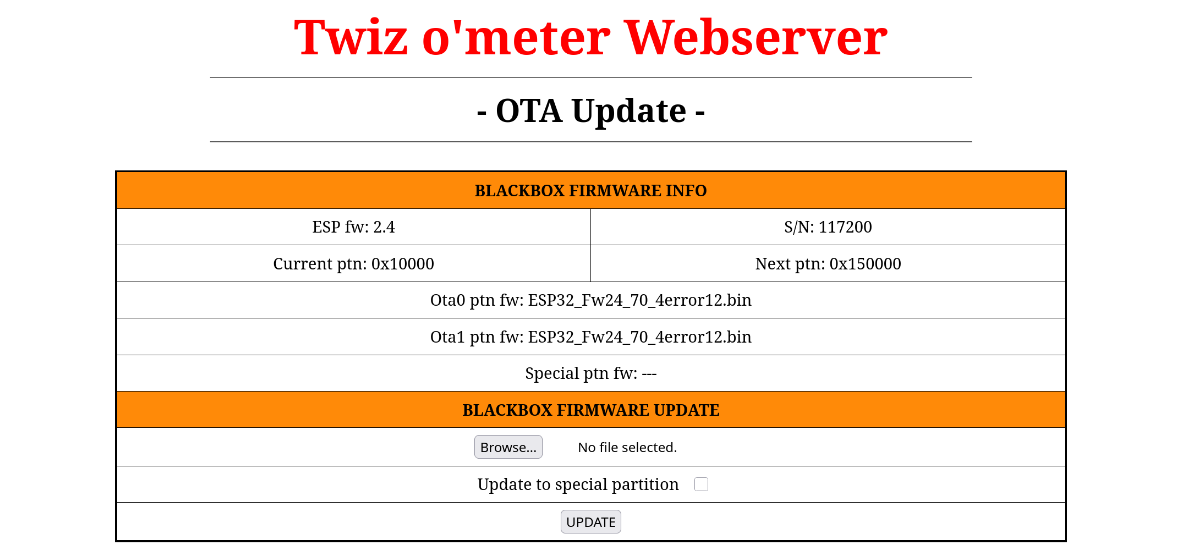
\includegraphics[width=1\textwidth]{figures/ota_page3.png}
    \caption{OTA Update page --- Update and info table.}
\end{figure}

When the update progress bar reaches 100\%, ToM+ LCD display will become black and 
that is the successful sign that ToM+ is rebooting, loading the \textit{Twizy-cfg} software.
Now, you need to connect to \textbf{“Twizy-cfg”} access point on your device to access
its webserver and if requested, accept to keep the connection active even if
it doesn't provide an Internet access.

The \textbf{password} is the default ToM+ password, which is the word “pass” followed by your 
device serial number (e.g. \textit{pass129777}). Serial number can be found in the 
settings page as explained in Figure~\ref{fig:settings_page}.\\

Now, open a web browser and type \textbf{192.168.4.1/webserial} to navigate to the
web server interface, where you can send tuning commands. The command terminal looks
like the one shown in the image here. As already said, tuning isn't an official ToM+
feature and \textit{Twizy-cfg} wasn't written by me, so please refer to \href{https://www.twizy-forum.de/projekte-twizy/83451-twizy-cfg-sevcon-shell-fuer-arduino?start=0}{Twizy-cfg topic}
or to its \href{https://github.com/dexterbg/Twizy-Cfg}{Github repository} to know 
tuning commands and configurations.\\

\begin{figure}[H]
    \centering
    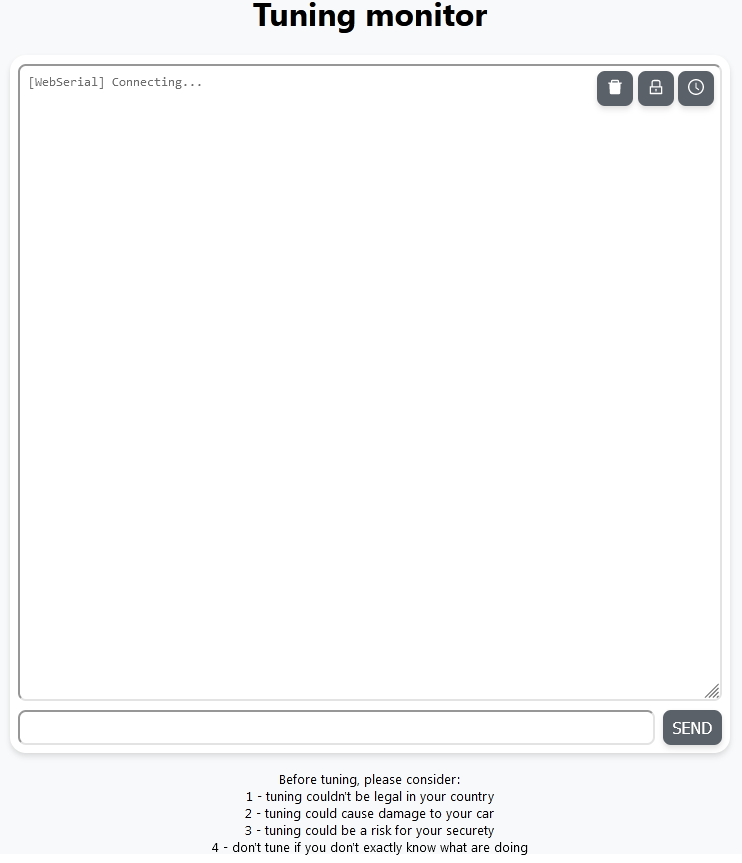
\includegraphics[width=0.7\textwidth]{figures/TuningMonitor.PNG}
    \caption{Tuning monitor to perform tuning commands.}
\end{figure}

As long as you are using Twizy-cfg, ToM+ firmware won't be loaded and so the display
won't power on. When you want to get back to official ToM+ firmware, you will just
need to type in the tuning monitor this self-explanatory command: \textbf{reboot}.\\

And that's it, ToM+ reboots to the other partition and gets back to its normal
behaviour and the tuning configuration will persist in your Twizy. The next time
you will need the Twizy-cfg shell, just go in the \textbf{“OTA Update and Prefs”}
page on ToM+ web server and select the option \textit{“REBOOT FROM SPECIAL PARTITION”}
from the table shown in the next image. No need to upload the \textit{“.bin”} file again.

\begin{figure}[H]
    \centering
    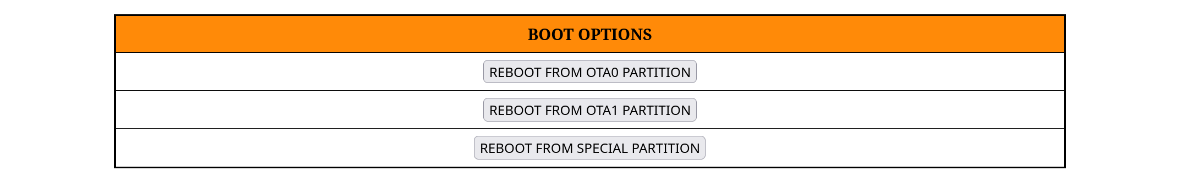
\includegraphics[width=1\textwidth]{figures/ota_boot.png}
    \caption{OTA Update page --- Boot options table.}
\end{figure}


\chapter{Controlling Tasmota WiFi switch}
\label{apx:tasmota}

\section{What are WiFi switches/plugs?}

In this appendix I'll explain how you can configure your ToM+ to interact with a WiFi
AC switch / AC plug, or any other device running a \textbf{Tasmota firmware}.

Basicaly they are \textit{relais modules} which can be controlled remotly via a wireless connection.
You can easly find this sort of devices on lots of e-commerce websites (like Amazon),
for a few tens of euros.\\

They have many formats, but frequently they appear in the two shown in the image.
The second one is more compact and user-friendly, while the first one needs some 
cable connection to work with your electric equipments.

\begin{figure}[ht]
    \centering
    \begin{subfigure}[t]{0.48\textwidth}
        \centering
        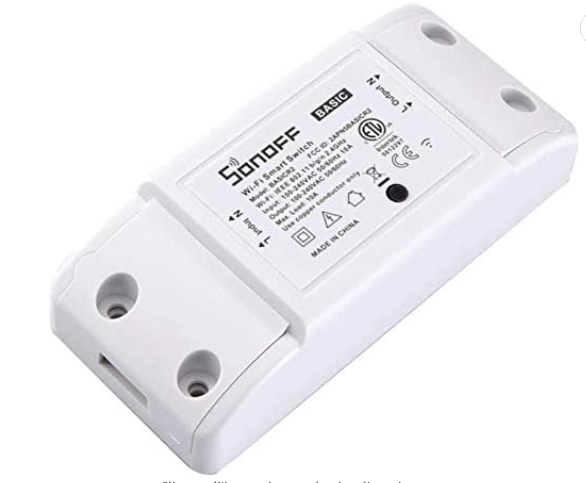
\includegraphics[width=\linewidth]{figures/Sonoff.PNG}
        \caption{Sonoff WiFi smart switch.}
    \end{subfigure}
    \hfill
    \begin{subfigure}[t]{0.48\textwidth}
        \centering
        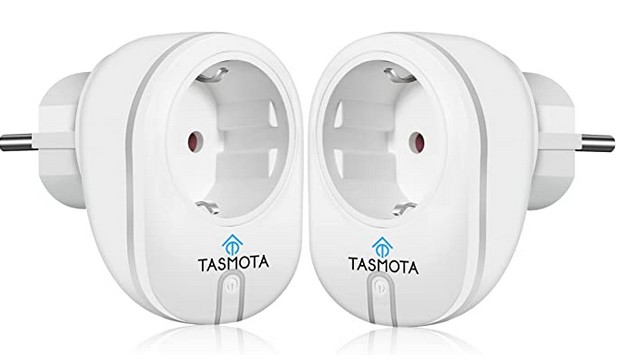
\includegraphics[width=\linewidth]{figures/TasmotaPlug.PNG}
        \caption{Tasmota WiFi smart plug.}
    \end{subfigure}
\end{figure}

\textit{But why is this useful?} There are many reasons you could need ToM+ connected to these devices.
Let's say: you want to stop traction battery charging if the charger is overheated and
restart charging when the temperature decreases; or maybe you want to \textbf{stop charging}
when a desired SOC is reached.

Or, like I did in this appendix with experimental purposes, to light on a lamp in my 
room when Twizy (parked in the garage) has almost completed charging.
In short, there are plenty of useful ideas where a WiFi switch/plug along with
ToM+ can help, creating nice projects.


\section{Requirements before starting}

To achieve this goal you will need a black box running a firmware version \textbf{1.4}
or above. This is a crucial requirement, because this process needs
features that were introduced in the mentioned version. See Section~\ref{sec:settings_page}
to check your ESP firmware version and Section~\ref{sec:web_ota_update} to update your
firmware via OTA if needed.

Additionally, you will need to have \textbf{WiFi and MQTT configured} to make the whole system
work. If not, please refer to Section~\ref{sec:wifi_settings} to set up WiFi and to
Section~\ref{sec:mqtt_connection} for the MQTT configuration. They must be both 
enabled and connected to accomplish this task.\\

Then, you will obviously need a wireless switch or plug, depending on your needs and
it must be running a \textbf{Tasmota firmware} (\textit{version 7} or above).

Bear in mind that \textit{“Sonoff”} like devices come out the fabric with a proprietary
firmware which doesn't natively support MQTT protocol.\\

In order to use them, as I did in this appendix, you have to upgrade them to Tasmota firmware.
Web is full of guides about installing Tasmota firmware, so look for the one that
suits your device and follow it.
For users who don't want to face with firmware update procedure, I personally suggest
to buy a device already running Tasmota firmware.


\section{Tasmota MQTT configuration}

Navigate to the \textbf{Tasmota WebUI} and you will get a landing page similar to the one
show below. At any time, if unsure, please refer to the \href{https://tasmota.github.io/docs/}{official documentation}.

\begin{figure}[H]
    \centering
    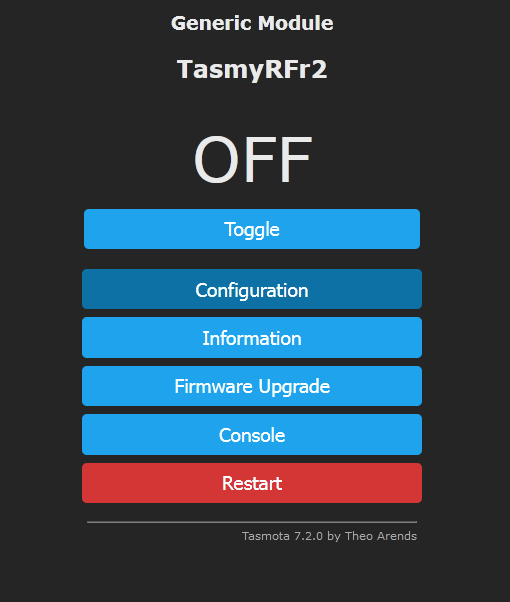
\includegraphics[width=0.45\textwidth]{figures/Mqtt1.PNG}
    \caption{Tasmota webUI --- Landing page.}
\end{figure}

First of all, press the \textbf{“Configuration”} button that will take you to the page shown
in the first image below.
After that, configure the \textit{WiFi connection}, entering your parameters (SSID and password) in
Tasmota's \textbf{“Configure WiFi”} page. Then, follow the instruction to configure 
\textit{MQTT settings}, accessing \textbf{“Configure MQTT”} webUI page.\\

\clearpage

\begin{figure}[ht]
    
    \begin{subfigure}[t]{0.4\textwidth}
        \centering
        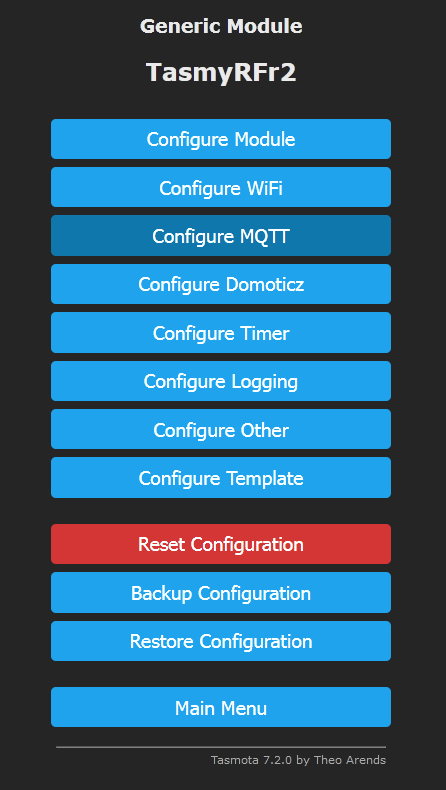
\includegraphics[width=\linewidth]{figures/Mqtt2.PNG}
        \caption{Configuration page.}
    \end{subfigure}
    \hfill
    \begin{subfigure}[t]{0.48\textwidth}
        \centering
        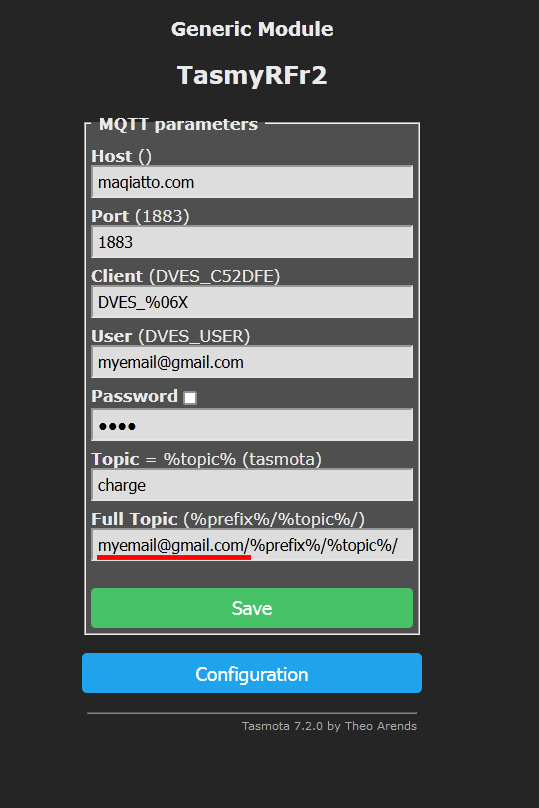
\includegraphics[width=\linewidth]{figures/Mqtt4.PNG}
        \caption{MQTT configuration page.}
    \end{subfigure}
\end{figure}

Now enter your broker address, user ID, password and port number. They must be the same
set on ToM+! You can check the explanation for each field in Section~\ref{sec:mqtt_connection}.\\

The most difficult parameters to understand are \textbf{“Topic”} and \textbf{“Full Topic”}.
These must not be the same as ToM+ MQTT topics, because they are specific for the device you are using.
If you put the same \textit{TOMin} and \textit{TOMout} topics the communications may 
disturb each other.\\

In the first field enter whatever you want. I suggest something that reminds your 
device function. But please use a short string (5/6 chars are enough), because this
field will be a minimal part of the full topic string and ToM+ has a limit of 50 chars
for \textbf{“Auxilliary MQTT command”} field (discussed in Section~\ref{sec:web_alarm_triggers}).

In the second field, it's important to distinguish between two options, depending on
which broker you are using. If you have your own broker (i.e. \textit{not Maqiatto}),
then leave the default string \textbf{\%prefix\%/\%topic\%/}.\\

If you use Maqiatto instead, configured following Section~\ref{sec:free_broker} or 
any another broker which adds \textit{your email as a prefix} of the topic name, then
edit the \textbf{“Full Topic”} field accordingly. \linebreak The fields will be the one shown 
in the second image above, so it becomes \linebreak \textbf{myemail@gmail.com/\%prefix\%/\%topic\%/},
adding your userID (email) as a prefix.

Finally, press the \textbf{“Save”} green button and wait until the device reboots.\\

\textbf{REMEMBER!} If you are using Maqiatto broker, you may need to add the new topic
to your account as explained in Figure~\ref{sec:free_broker_add_topics}.

In this case, you'll have to add \textbf{cmnd/<your\textunderscore~Tasmota\textunderscore~topic\textunderscore~name>/Power} as the new topic name,
that will become \textit{cmnd/charge/Power} if you followed the image.


\section{ToM+ Tasmota configuration}

Open ToM+ webserver as explained in Section~\ref{sec:web_server_access} and go to the
\textbf{“Alarm triggers”} page. Now, add a new allarm to the list accordingly to the
item which will control your Tasmota device, as explained in Section~\ref{sec:web_alarm_triggers}.

In my case, I chose \textbf{“Battery SOC”} item, that will trigger alarm when its 
value will be \textit{equal to 97\%}, to notify the quite completed charge.

\begin{figure}[H]
    \centering
    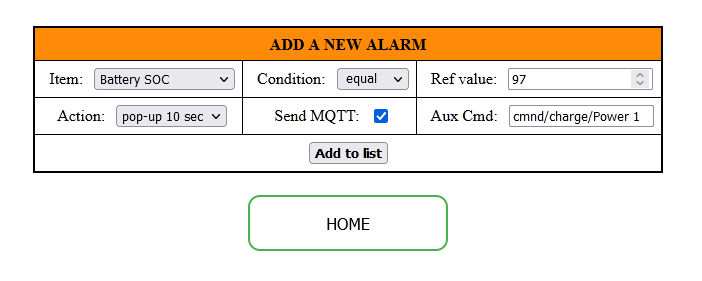
\includegraphics[width=0.7\textwidth]{figures/Tom01.PNG}
    \caption{Adding the Tasmota trigger on ToM+.}
\end{figure}

As you may notice, the most important part is to configure properly the \textbf{“Aux Cmd”}
field, because it contains the control MQTT command that ToM+ will send to 
the Tasmota device.

If you have your own MQTT broker (i.e. \textit{not Maqiatto}) the \textbf{Aux Cmd} will have this syntax:
\begin{itemize}
    \item \textit{cmnd/<your\textunderscore~Tasmota\textunderscore~topic\textunderscore~name>/Power 1} if you want to power ON the device.
    \item \textit{cmnd/<your\textunderscore~Tasmota\textunderscore~topic\textunderscore~name>/Power 0} if you want to power it OFF.
\end{itemize}
Again, in our example the command becomes \textbf{cmnd/charge/Power 1} to power the lamp ON.\\

Otherwise, if you are using Maqiatto broker or another one which uses your userID (e-mail)
as a prefix in topics name, then the \textbf{Aux Cmd} syntax will look in this other way:
\begin{itemize}
    \item \textit{myemail@gmail.com/cmnd/<your\textunderscore~Tasmota\textunderscore~topic\textunderscore~name>/Power 1} to power it ON.
    \item \textit{myemail@gmail.com/cmnd/<your\textunderscore~Tasmota\textunderscore~topic\textunderscore~name>/Power 0} to power it OFF.
\end{itemize}
In our case, the command becomes \textbf{myemail@gmail.com/cmnd/charge/Power 1}.\\

If you want to stop charging and then restart when specific conditions are met, you
need to add two alarms, one for each Power ON/OFF condition, using the explained syntax accordingly.\\

Please note that, if you have a device with more relais, you will have to 
edit the above syntax specifying which relais you want to control: using \textbf{“Power1”}
for the first relay, \textbf{“Power2”} for the second one and so on. This becomes:
\begin{itemize} 
    \item \textit{cmnd/<your\textunderscore~Tasmota\textunderscore~topic\textunderscore~name>/Power1 1} to power ON the first relay.
    \item \textit{cmnd/<your\textunderscore~Tasmota\textunderscore~topic\textunderscore~name>/Power1 0} to power it OFF.
\end{itemize}
The same syntax distinction about Maqiatto and owned brokers applies here as well.

\section{Common problems and fixes}

Some Tasmota firmwares don't like \textit{Maqiatto} topic format, so if you want to 
drive a Tasmota device with ToM+, you have to use another MQTT broker.
After some tests, I noticed you can use successfuly use \href{https://dealgate.ru/}{mqtt.dealgate.ru},
free and more features-rich. 

The downside is that you have to face with some russian translations to create the account.
But nothing than an online translator cannot do.